% Options for packages loaded elsewhere
\PassOptionsToPackage{unicode}{hyperref}
\PassOptionsToPackage{hyphens}{url}
%
\documentclass[
  12pt,
]{article}
\usepackage{lmodern}
\usepackage{amssymb,amsmath}
\usepackage{ifxetex,ifluatex}
\ifnum 0\ifxetex 1\fi\ifluatex 1\fi=0 % if pdftex
  \usepackage[T1]{fontenc}
  \usepackage[utf8]{inputenc}
  \usepackage{textcomp} % provide euro and other symbols
\else % if luatex or xetex
  \usepackage{unicode-math}
  \defaultfontfeatures{Scale=MatchLowercase}
  \defaultfontfeatures[\rmfamily]{Ligatures=TeX,Scale=1}
\fi
% Use upquote if available, for straight quotes in verbatim environments
\IfFileExists{upquote.sty}{\usepackage{upquote}}{}
\IfFileExists{microtype.sty}{% use microtype if available
  \usepackage[]{microtype}
  \UseMicrotypeSet[protrusion]{basicmath} % disable protrusion for tt fonts
}{}
\makeatletter
\@ifundefined{KOMAClassName}{% if non-KOMA class
  \IfFileExists{parskip.sty}{%
    \usepackage{parskip}
  }{% else
    \setlength{\parindent}{0pt}
    \setlength{\parskip}{6pt plus 2pt minus 1pt}}
}{% if KOMA class
  \KOMAoptions{parskip=half}}
\makeatother
\usepackage{xcolor}
\IfFileExists{xurl.sty}{\usepackage{xurl}}{} % add URL line breaks if available
\IfFileExists{bookmark.sty}{\usepackage{bookmark}}{\usepackage{hyperref}}
\hypersetup{
  pdftitle={Econometrics II TA Session \#1},
  pdfauthor={Hiroki Kato},
  hidelinks,
  pdfcreator={LaTeX via pandoc}}
\urlstyle{same} % disable monospaced font for URLs
\usepackage[margin=1in]{geometry}
\usepackage{color}
\usepackage{fancyvrb}
\newcommand{\VerbBar}{|}
\newcommand{\VERB}{\Verb[commandchars=\\\{\}]}
\DefineVerbatimEnvironment{Highlighting}{Verbatim}{commandchars=\\\{\}}
% Add ',fontsize=\small' for more characters per line
\usepackage{framed}
\definecolor{shadecolor}{RGB}{248,248,248}
\newenvironment{Shaded}{\begin{snugshade}}{\end{snugshade}}
\newcommand{\AlertTok}[1]{\textcolor[rgb]{0.94,0.16,0.16}{#1}}
\newcommand{\AnnotationTok}[1]{\textcolor[rgb]{0.56,0.35,0.01}{\textbf{\textit{#1}}}}
\newcommand{\AttributeTok}[1]{\textcolor[rgb]{0.77,0.63,0.00}{#1}}
\newcommand{\BaseNTok}[1]{\textcolor[rgb]{0.00,0.00,0.81}{#1}}
\newcommand{\BuiltInTok}[1]{#1}
\newcommand{\CharTok}[1]{\textcolor[rgb]{0.31,0.60,0.02}{#1}}
\newcommand{\CommentTok}[1]{\textcolor[rgb]{0.56,0.35,0.01}{\textit{#1}}}
\newcommand{\CommentVarTok}[1]{\textcolor[rgb]{0.56,0.35,0.01}{\textbf{\textit{#1}}}}
\newcommand{\ConstantTok}[1]{\textcolor[rgb]{0.00,0.00,0.00}{#1}}
\newcommand{\ControlFlowTok}[1]{\textcolor[rgb]{0.13,0.29,0.53}{\textbf{#1}}}
\newcommand{\DataTypeTok}[1]{\textcolor[rgb]{0.13,0.29,0.53}{#1}}
\newcommand{\DecValTok}[1]{\textcolor[rgb]{0.00,0.00,0.81}{#1}}
\newcommand{\DocumentationTok}[1]{\textcolor[rgb]{0.56,0.35,0.01}{\textbf{\textit{#1}}}}
\newcommand{\ErrorTok}[1]{\textcolor[rgb]{0.64,0.00,0.00}{\textbf{#1}}}
\newcommand{\ExtensionTok}[1]{#1}
\newcommand{\FloatTok}[1]{\textcolor[rgb]{0.00,0.00,0.81}{#1}}
\newcommand{\FunctionTok}[1]{\textcolor[rgb]{0.00,0.00,0.00}{#1}}
\newcommand{\ImportTok}[1]{#1}
\newcommand{\InformationTok}[1]{\textcolor[rgb]{0.56,0.35,0.01}{\textbf{\textit{#1}}}}
\newcommand{\KeywordTok}[1]{\textcolor[rgb]{0.13,0.29,0.53}{\textbf{#1}}}
\newcommand{\NormalTok}[1]{#1}
\newcommand{\OperatorTok}[1]{\textcolor[rgb]{0.81,0.36,0.00}{\textbf{#1}}}
\newcommand{\OtherTok}[1]{\textcolor[rgb]{0.56,0.35,0.01}{#1}}
\newcommand{\PreprocessorTok}[1]{\textcolor[rgb]{0.56,0.35,0.01}{\textit{#1}}}
\newcommand{\RegionMarkerTok}[1]{#1}
\newcommand{\SpecialCharTok}[1]{\textcolor[rgb]{0.00,0.00,0.00}{#1}}
\newcommand{\SpecialStringTok}[1]{\textcolor[rgb]{0.31,0.60,0.02}{#1}}
\newcommand{\StringTok}[1]{\textcolor[rgb]{0.31,0.60,0.02}{#1}}
\newcommand{\VariableTok}[1]{\textcolor[rgb]{0.00,0.00,0.00}{#1}}
\newcommand{\VerbatimStringTok}[1]{\textcolor[rgb]{0.31,0.60,0.02}{#1}}
\newcommand{\WarningTok}[1]{\textcolor[rgb]{0.56,0.35,0.01}{\textbf{\textit{#1}}}}
\usepackage{graphicx}
\makeatletter
\def\maxwidth{\ifdim\Gin@nat@width>\linewidth\linewidth\else\Gin@nat@width\fi}
\def\maxheight{\ifdim\Gin@nat@height>\textheight\textheight\else\Gin@nat@height\fi}
\makeatother
% Scale images if necessary, so that they will not overflow the page
% margins by default, and it is still possible to overwrite the defaults
% using explicit options in \includegraphics[width, height, ...]{}
\setkeys{Gin}{width=\maxwidth,height=\maxheight,keepaspectratio}
% Set default figure placement to htbp
\makeatletter
\def\fps@figure{htbp}
\makeatother
\setlength{\emergencystretch}{3em} % prevent overfull lines
\providecommand{\tightlist}{%
  \setlength{\itemsep}{0pt}\setlength{\parskip}{0pt}}
\setcounter{secnumdepth}{5}
\usepackage{zxjatype}
\setCJKmainfont[BoldFont = IPAゴシック]{IPA明朝}
\setCJKsansfont{IPAゴシック}
\setCJKmonofont{IPAゴシック}
\parindent = 1em
\newcommand{\argmax}{\mathop{\rm arg~max}\limits}
\newcommand{\argmin}{\mathop{\rm arg~min}\limits}
\DeclareMathOperator*{\plim}{plim}
\usepackage{xcolor}
\ifluatex
  \usepackage{selnolig}  % disable illegal ligatures
\fi
\newlength{\cslhangindent}
\setlength{\cslhangindent}{1.5em}
\newenvironment{cslreferences}%
  {\setlength{\parindent}{0pt}%
  \everypar{\setlength{\hangindent}{\cslhangindent}}\ignorespaces}%
  {\par}

\title{Econometrics II TA Session \#1}
\author{Hiroki Kato}
\date{}

\begin{document}
\maketitle

\hypertarget{about-ta-session}{%
\section{About TA Session}\label{about-ta-session}}

\begin{itemize}
\tightlist
\item
  Class schedule: Friday pm 13:30-15:00 via zoom.

  \begin{itemize}
  \tightlist
  \item
    You can access the meeting ID and its pascode via CLE.
  \end{itemize}
\item
  Instructor (If you have any question, please contact us via e-mail)

  \begin{enumerate}
  \def\labelenumi{\arabic{enumi}.}
  \tightlist
  \item
    Hiroki Kato (D2,
    \href{mailto:vge008kh@student.econ.osaka-u.ac.jp}{\nolinkurl{vge008kh@student.econ.osaka-u.ac.jp}})
  \item
    Pang Kan (D1,
    \href{mailto:member_1363710747@yahoo.co.jp}{\nolinkurl{member\_1363710747@yahoo.co.jp}})
  \end{enumerate}
\item
  Purpose: We will review the contents of the main class ``Econometics
  II." using R which is a free software environment for statistical
  computing.

  \begin{itemize}
  \tightlist
  \item
    We strongly recommend that you download R
    (\url{https://www.r-project.org/}) and its IDE called R studio
    (\url{https://rstudio.com/products/rstudio/download/}), and try to
    reproduct by yourself.
  \end{itemize}
\end{itemize}

\hypertarget{review-matrix-algebra}{%
\section{Review: Matrix Algebra}\label{review-matrix-algebra}}

\hypertarget{addition-and-subtraction}{%
\subsection{Addition and Subtraction}\label{addition-and-subtraction}}

Consider \(A = (a_{ij}) \in \mathbb{R}^{m \times n}\) and
\(B = (b_{ij}) \in \mathbb{R}^{p \times q}\). Addition and subtraction
require that the dimentions are same, that is, \(m = p\) and \(n = q\).
Then, the sum of two matricies is \begin{align*}
  A + B = (a_{ij} + b_{ij}).
\end{align*} The difference of two matricies is \begin{align*}
  A - B = (a_{ij} - b_{ij}).
\end{align*}

\hypertarget{multiplication}{%
\subsection{Multiplication}\label{multiplication}}

The standard matrix multiplication requires that the number of columns
of the first matrix is equal to the number of rows of the second matrix
(\(n = p = l\)). The product of two matricies is \begin{align*}
  AB = (\sum_{k=1}^l a_{ik} b_{kj}) \in \mathbb{R}^{m \times q}.
\end{align*} We should remark following important points about
multiplication:

\begin{itemize}
\tightlist
\item
  it holds non-commutativity: \(XY \not= YX\);
\item
  it holds associative law: \((XY)Z = X(YZ)\);
\item
  it holds distributive law: \(X(Y + Z) = XY + XZ\);
\item
  when \(B = A\), we obtain the second power of a matrix \(A\), that is,
  \(A^2 = A A\). Especially, if a martix \(A\) holds \(AA = A\), then
  the matrix is called an \textbf{idempotent matrix (べき等行列)}.
\end{itemize}

We introduce the another key product of matrix, called the
\textbf{Kronecker product (クロネッカー積)}. This is defined by
\begin{align*}
  A \otimes B = (a_{ij} B) \in \mathbb{R}^{mp \times nq}.
\end{align*} The Kronecker product has a following property:

\begin{itemize}
\tightlist
\item
  \(X_{1}X_{2} \otimes Y_{1}Y_{2} = (X_{1} \otimes Y_{1})(X_{2} \otimes Y_{2})\)
\end{itemize}

\hypertarget{transposed-matrix-diagonal-matrix-and-inverse-matrix}{%
\subsection{Transposed Matrix, Diagonal Matrix, and Inverse
Matrix}\label{transposed-matrix-diagonal-matrix-and-inverse-matrix}}

Consider \(X = (x_{ij}) \in \mathbb{R}^{m \times n}\) throughout this
subsection.

\hypertarget{transposed-matrix.}{%
\subsubsection{Transposed Matrix.}\label{transposed-matrix.}}

The \textbf{transposed matrix (転置行列)} of \(X\), denoted by \(X'\) is
a \(n \times m\) matrix whose element \(x'_{ij}\) holds \begin{align*}
  x'_{ij} = x_{ji}.
\end{align*} That is, \(i\)-th row and \(j\)-th column element of
transposed matrix is \(j\)-th row and \(i\)-th column element of
original matrix. We remark following important points:

\begin{itemize}
\tightlist
\item
  it holds \((XY)' = Y'X'\);
\item
  it holds \((XYZ)' = Z'Y'X'\);
\item
  \((X \otimes Y)' = X' \otimes Y'\);
\item
  let \(x_i = (x_{i1}, \ldots x_{ij})\) be a row vector of matrix \(X\).
  Then, we have \(X'X = \sum_{n = 1}^i x'_n x_n\);
\item
  if a matrix \(X\) holds \(X' = X\), then the matrix is called a
  \textbf{symmetric matrix (対称行列)}.
\end{itemize}

\hypertarget{diagonal-matrix-and-trace}{%
\subsubsection{Diagonal Matrix and
Trace}\label{diagonal-matrix-and-trace}}

Suppose a matrix \(X\) is a \textbf{square matrix (正方行列)}, that is,
\(n = m\). The matrix \(X\) is called a \textbf{diagonal matrix
(対角行列)} whose diagonal elements (\(i\)-th row and \(i\)-th column
elements) consist of \((x_{11}, \ldots x_{nn})\), and other elements are
zero. That is, \begin{align*}
  X 
  = diag(x_{11}, x_{22}, \ldots, x_{ii})
  =
  \begin{pmatrix}
    x_{11} & 0 & 0 & \cdots & 0 \\
    0 & x_{22} & 0 & \cdots & 0 \\
    \vdots & \vdots & \vdots & \vdots & \vdots \\
    0 & 0 & 0 & \cdots & x_{nn}
  \end{pmatrix}.
\end{align*} Especially, a matrix \(I = diag(1, 1, \ldots, 1)\) is
called an \textbf{identity matrix (単位行列)}.

There is one important concept, called \textbf{trace (トレース)},
related with diagonal elements of matrix. The trace of matrix is derived
by the sum of diagonal elements, that is, \begin{align*}
  tr(X) = \sum_{n = 1}^{i} x_{nn}.
\end{align*} The trace has following properties:

\begin{itemize}
\tightlist
\item
  \(tr(cX) = c \cdot tr(X)\) where \(c\) is scalar;
\item
  \(tr(X') = tr(X)\);
\item
  \(tr(X + Y) = tr(X) + tr(Y)\);
\item
  \(tr(XY) = tr(YX)\);
\item
  \(xx' = tr(x'x) = tr(x x')\) if \(x\) is a \(1 \times j\) vector.
\end{itemize}

\hypertarget{inverse-matrix}{%
\subsubsection{Inverse Matrix}\label{inverse-matrix}}

the matrix \(X\) is \textbf{regular matrix (正則行列)} if there exists a
matrix \(Y\) such that \begin{align*}
  X Y = I,
\end{align*} where \(I\) is an identity matrix. In this case, the matrix
\(Y\) is called an \textbf{inverse matrix (逆行列)}, which is denoted by
\(X^{-1}\). The inverse matrix has following important properties:

\begin{itemize}
\tightlist
\item
  \((X^{-1})' = (X')^{-1}\);
\item
  \((X \otimes Y)^{-1} = X^{-1} \otimes Y^{-1}\) if the inverse exists;
\item
  \((X \otimes Y)(X^{-1} \otimes Y^{-1}) = I\)
\end{itemize}

\hypertarget{quadratic-forms}{%
\subsection{Quadratic Forms}\label{quadratic-forms}}

Consider a symmetric and square matrix \(A \in \mathbb{R}^{n \times n}\)
and a vector \(x \in \mathbb{R}^{n \times 1}\). Then, the quadratic form
is written as \begin{align*}
  Q = x' A x.
\end{align*} For example, consider \(x = (x, y)'\) and \(A\) is a
\(2 \times 2\) matrix whose elements is one. Then, the quadratic form is
\begin{align*}
  Q 
  =
  \begin{pmatrix} x & y \end{pmatrix}
  \begin{pmatrix} 1 & 1 \\ 1 & 1 \end{pmatrix}
  \begin{pmatrix} x \\ y \end{pmatrix}
  =
  \begin{pmatrix} x+y & x+y \end{pmatrix}
  \begin{pmatrix} x \\ y \end{pmatrix}  
  = x^2 + 2xy + y^2 = (x + y)^2.
\end{align*} In this case, for any non-zero \(x\) and \(y\), \(Q\) takes
non-negative value. Then, we call the matrix \(A\) \emph{positive
semidefinite}. The definiteness of matrix is defined as follows:

\begin{itemize}
\tightlist
\item
  If \(x'Ax > 0\) for all nonzero \(x\), then \(A\) is \textbf{positive
  definite (正値定符号)}.
\item
  If \(x'Ax < 0\) for all nonzero \(x\), then \(A\) is \textbf{negative
  definite (負値定符号)}.
\item
  If \(x'Ax \ge 0\) for all nonzero \(x\), then \(A\) is
  \textbf{positive semidefinite (半正値定符号)}.
\item
  If \(x'Ax \le 0\) for all nonzero \(x\), then \(A\) is
  \textbf{negative semidefinite(半負値定符号)}.
\end{itemize}

\hypertarget{characteristic-roots-and-characteristic-vectors}{%
\subsubsection{Characteristic Roots and Characteristic
Vectors}\label{characteristic-roots-and-characteristic-vectors}}

Before describing useful theorm to check definiteness easily, we have to
introduce two concepts: \textbf{characteristic roots (固有根)} and
\textbf{characteristic vectors (固有ベクトル)}.

\begin{quote}
If a scalar \(\lambda\) and a vector \(c\in \mathbb{R}^{k \times 1}\),
which is normalized as \(c'c=1\), satisfy the following equation, then
they are called as the \textbf{characteristic root} and the
\textbf{characteristic vector}, respectively; \begin{align*}
Ac=\lambda c \Leftrightarrow (A-\lambda I)c = 0,
\end{align*} where \(I\) is an identity matrix.
\end{quote}

These (\(\lambda_1,\lambda _2,...,\lambda _k\)) correspond to
characteristic vectors \((c_1, c_2, \dots ,c_k)\). There is the
following useful theorm that states the relationship between
characteristic roots and definiteness:

\begin{quote}
Let \(A\) be a symmetric matrix.

\begin{enumerate}
\def\labelenumi{\arabic{enumi}.}
\tightlist
\item
  If all the characteristic roots of \(A\) are positive (negative), then
  \(A\) is positive definite (negative definite).
\item
  If some of roots are zero, then \(A\) is positive (negative)
  semidefinite if the reminder are positive (negative).
\item
  If \(A\) has both negative and positive roots, then \(A\) is
  indefinite.
\end{enumerate}
\end{quote}

\hypertarget{determinants}{%
\subsubsection{Determinants}\label{determinants}}

Alternative way to check definiteness of matrix is to using
\textbf{determinants (行列式)}, which is a scalar quantity defined by a
square matrix \(A = (a_{ij}) \in \mathbb{R}^{n \times n}\). The
determinant of \(2 \times 2\) matrix, i.e., \(n = 2\), is obtained by
\begin{align*}
  det(A) = a_{11}a_{22} - a_{12}a_{21}.
\end{align*} Using the determinant of a matrix with \(n = 2\), we can
calculate the determinant of \(3 \times 3\) matrix. Let \(det(A_{ij})\)
be the determinant of the \(2 \times 2\) submatrix obtained when
\(i\)-th row and \(j\)-th column are removed from the original matrix,
which is called \textbf{minor (小行列式)}. Furthermore, we define
\(C_{ij} = (-1)^{i+j} det(A_{ij})\), which is called \textbf{cofactor
(余因子)}. We call a matrix in which each element \(a_{ij}\) is replaced
by the corresponding cofactor \(C_{ij}\) \textbf{cofactor matrix
(余因子行列)}. Then, the determinant of \(3 \times 3\) matrix is
\begin{align*}
  det(A) 
  &= a_{11} C_{11} + a_{12} C_{12} + a_{13} C_{13}  \\
  &= a_{11} 
  \left| \begin{array}{cc}
    a_{22} & a_{23} \\
    a_{32} & a_{33}
  \end{array} \right| 
  - a_{12}
  \left| \begin{array}{cc}
    a_{21} & a_{23} \\
    a_{31} & a_{33}
  \end{array} \right| 
  + a_{13}
  \left| \begin{array}{cc}
    a_{21} & a_{22} \\
    a_{31} & a_{32}
  \end{array} \right|, 
\end{align*} or \begin{align*}
  det(A) = a_{11} C_{11} + a_{21} C_{21} + a_{31} C_{31}.
\end{align*} How about matrices with \(n \ge 4\)? Essentially, we can
calculate the determinant, using cofactors. That is, for any \(i\),
\begin{align*}
  det(A) = \sum_{k = 1}^n a_{ik} C_{ik},
\end{align*} or, for any \(j\) \begin{align*}
  det(A) = \sum_{k = 1}^n a_{kj} C_{kj},
\end{align*}

Before describing the important theorem to check definiteness, we
introduce the \emph{Cramer's rule}, which provides inverse matrices.

\begin{quote}
Let \(A \in \mathbb{R}^{n \times n}\) be a square matrix with
\(det(A) \not= 0\). Then, the inverse matrix of \(A\) is equal to the
transposed cofactor matrix multiplied by \(det(A)^{-1}\). That is,
\begin{align*}
A^{-1} = \frac{1}{det(A)} 
\begin{pmatrix}
C_{11} & \cdots & C_{n1} \\
\vdots & \vdots & \vdots \\
C_{1n} & \cdots & C_{nn}
\end{pmatrix}. 
\end{align*}
\end{quote}

Next, we introduce the useful theorem to check definiteness of
matricies. The determinant has the follwoing relation with the
definiteness of matricies.

\begin{quote}
Let \(A \in \mathbb{R}^{n \times n}\) be a square matrix. Let
\begin{align*}
det(A_i) = 
\left| \begin{array}{ccc}
a_{11} & \cdots & a_{1i} \\
\vdots & \vdots & \vdots \\
a_{i1} & \cdots & a_{ii}
\end{array} \right|. 
\end{align*} A necessary and sufficient condition for a matrix A to be
positive definite is that \(det(A_i) > 0\) for all
\(i \in \{1, \ldots, n\}\). Moreover, a necessary sufficient condition
for a matrix A to be negative definite is that \(det(A_i) < 0\) for odd
\(i\) and \(det(A_i) > 0\) for even \(i\).
\end{quote}

As an illustration, consider the following matrix: \begin{align*}
  A = 
  \begin{pmatrix}
    6 & 4 \\
    4 & 5
  \end{pmatrix}.
\end{align*} Then, we have \(det(A_1) = 6 > 0\) and
\(det(A_2) = 30 - 16 > 0\). Thus, this matrix is positive definite.

To show another example, we use the following diagonal matrix:
\begin{align*}
  A = 
  \begin{pmatrix}
    -3 & 0 & 0 \\
    0 & -2 & 0 \\
    0 & 0 & -1
  \end{pmatrix}.
\end{align*} Since the determinant of a diagonal matrix can be computed
as the product of diagonal elements, we have \(det(A_1) = -3\),
\(det(A_2) = (-3)(-2) = 6 > 0\), and
\(det(A_3) = (-3)(-2)(-1) = -6 < 0\). Thus, this diagonal matrix is
negative definite. Moreover, the inverse matrix of this diagonal matrix
is given by \begin{align*}
  A^{-1} = -\frac{1}{6}
  \begin{pmatrix}
    2 & 0 & 0 \\
    0 & 3 & 0 \\
    0 & 0 & 6
  \end{pmatrix}
  = 
  \begin{pmatrix}
    -1/3 & 0 & 0 \\
    0 & -1/2 & \\
    0 & 0 & -1
  \end{pmatrix}
\end{align*} Cleary, we have \(A A^{-1} = I\).

\hypertarget{differentiation}{%
\subsection{Differentiation}\label{differentiation}}

Consider two vectors: \(a \in \mathbb{R}^{n \times 1}\) and
\(x \in \mathbb{R}^{n \times 1}\). We obtain the product of transposed
vector of \(a\) and \(x\), that is,
\(a'x = a_1 x_1 + \cdots + a_n x_n\). Then, the differentiation of this
scalar with respect to \(x\) is defined by \begin{align*}
  \frac{\partial a'x}{\partial x}
  = 
  \begin{pmatrix} \frac{\partial a'x}{\partial x_1} \\ \vdots \\ \frac{\partial a'x}{\partial x_n} \end{pmatrix}
  = 
  a.
\end{align*}

Now, we expand to a symmetric and square matrix
\(A \in \mathbb{R}^{n \times n}\). Then, the differentiation of the
quadratic form \(x' A x\) with respect to \(x\) is defined by
\begin{align*}
  \frac{\partial x'Ax}{\partial x} = (A + A')x.
\end{align*}

\hypertarget{optimization}{%
\subsubsection{Optimization}\label{optimization}}

Consider function \(y = g(x)\) where \(x \in \mathbb{R}^{n}\), denoted
as \(g: \mathbb{R}^{n} \to \mathbb{R}\). We can obtain \(x^0\) such that
maximizing (minimizing) the function \(g\), using the following theorem:

\begin{quote}
If a function \(g \colon \mathbb{R}^{n} \rightarrow \mathbb{R}\) is
maximized (minimized) at the point
\(x^{0} = (x_{1}^{0}, \ldots, x_{n}^{0})\), then the following equation
holds: \begin{align*}
\frac{\partial g (x)}{\partial x} \Big{\vert}_{x = x^{0}} 
= 
\begin{pmatrix}
\frac{\partial g (x^{0})}{\partial x_{1}} \\
\vdots \\
\frac{\partial g (x^{0})}{\partial x_{n}} 
\end{pmatrix}  
= 0.
\end{align*} \(x^0\) is maximum (minimum) point if the following
\textbf{Hessian matrix (ヘッセ行列)} is negative (positive) definite:
\begin{align*}
H = \frac{\partial g (x)}{\partial xx'} 
=
\begin{pmatrix}
\frac{\partial^{2} g (x)}{\partial x_{1} \partial x_{1}} 
& \cdots & \frac{\partial^{2} g (x)}{\partial x_{1} \partial x_{n}} \\
\vdots  &\ddots  &\vdots\\
\frac{\partial^{2} g (x)}{\partial x_{n} \partial x_{1}} 
& \cdots & \frac{\partial^{2} g (x)}{\partial x_{n} \partial x_{n}}
\end{pmatrix}.
\end{align*}
\end{quote}

\hypertarget{review-probability}{%
\section{Review: Probability}\label{review-probability}}

This section refers to Wasserman (2013). Let \(\Omega\) be a
\textbf{(sample) space} which is the set of possible outcomes of an
experiment. Let \(\omega\) be \textbf{sample outcomes},
\textbf{reaizations}, or \textbf{elements}. Let \(A\) be \textbf{events}
which are the subsets of \(\Omega\). Then, we can define the
\textbf{probability} and \textbf{random variable} as follows:

\begin{quote}
A function \(\mathbb{P}\) that assigns a real number \(\mathbb{P}(A)\)
to each event A is a \textbf{probability} if it satisfies the following
three axioms:

\begin{enumerate}
\def\labelenumi{\arabic{enumi}.}
\tightlist
\item
  \(\mathbb{P}(A) \ge 0\) for all \(A\);
\item
  \(\mathbb{P}(\Omega) = 1\);
\item
  If \(A_1, A_2, \ldots\) are disjoint, then
  \(\mathbb{P}(\bigcup_{k=1}^{\infty}{A_k}) = \sum_{k=1}^{\infty} \mathbb{P}(A_i)\).
\end{enumerate}

A \textbf{random variable} is a mapping \(X: \Omega \to \mathbb{R}\)
that assigns a real number \(X(\omega)\) to each realization \(\omega\).
\end{quote}

For illustlation, consider the situation where you try to flip a fair
coin twice. Then, the sample space \(\Omega = \{ TT, HH, TH, HT \}\).
The probability of each outcome is 1/4, that is, \(P(\omega) = 1/4\) for
all \(\omega\). Let the random variable \(X\) be the number of heads.
Then, \(X(TT) = 0\), \(X(HH) = 2\), \(X(TH) = 1\), and \(X(HT) = 1\).

\hypertarget{distribution-functions}{%
\subsection{Distribution Functions}\label{distribution-functions}}

Given a random variable \(X\), we define \textbf{probability mass
function}, \textbf{probability density function} and \textbf{cumulative
distribution function} as follows:

\begin{quote}
Suppose that a random variable \(X\) is \emph{discrete} taking countably
many values \(\{x_1, \ldots\}\). Then, the \textbf{probability mass
function} for \(X\) is defined by \(f_X(x) = \mathbb{P}(X = x)\).

Suppose that a random variable \(X\) is \emph{continuous}. Then, there
exists a \textbf{probability density function} \(f_X\) such that (i)
\(f_X(x) \ge 0\) for all x, (ii)
\(\int_{-\infty}^{+\infty} f_X(x) dx = 1\) and (iii) for every
\(a \le b\), \(\mathbb{P}(a < X < b) = \int_a^b f_X(x)dx\).

The \textbf{cumulative distribution function (CDF)} is the function
\(F_X: \mathbb{R} \to [0, 1]\) defined by
\(F_X(x) = \mathbb{P}(X \le x)\).
\end{quote}

We summarize the relationship among three distribution functions as
follows: \begin{align*}
  F_X(x) =
  \begin{cases}
    \sum_{x_i \le x} f_X(x_i)  &\quad\text{$X$ is discrete} \\
    \int_{-\infty}^x f_X(t)dt  &\quad\text{$X$ is continuous}
  \end{cases}
\end{align*} From this, we obtain the property of CDF:

\begin{itemize}
\tightlist
\item
  \(F\) is non-decreasing: \(x_1 < x_2\) implies \(F(x_1) \le F(x_2)\);
\item
  \(F\) is normalized: \(\lim_{x \to -\infty} F(x) = 0\) and
  \(\lim_{x \to +\infty} F(x) = 1\);
\item
  \(F\) is right-contious: \(F(x) = F(x^+)\) for all \(x\), where
  \(F(x^+) = \lim_{y \downarrow x} F(y)\);
\item
  \(\mathbb{P}(X = x) = F(x) - F(x^-)\) where
  \(F(x^-) = \lim_{y \uparrow x} F(y)\);
\item
  \(\mathbb{P}(x < X \le y) = F(y) - F(x)\);
\item
  \(\mathbb{P}(X > x) = 1 - F(x)\).
\end{itemize}

\hypertarget{bivariate-distributions}{%
\subsubsection{Bivariate Distributions}\label{bivariate-distributions}}

When there are two random varibales, you can define bivariate
distributions as follows:

\begin{quote}
Given discrete random variables \(X\) and \(Y\), we define the
\textbf{joint mass function} by
\(f_{X,Y}(x, y) = \mathbb{P}(X = x, Y = y)\).
\end{quote}

\begin{quote}
In the continuous case, we call a function \(f(x, y)\) a \textbf{joint
probability density function} for the random variables \((X, Y)\) if (i)
\(f(x, y) \ge 0\), \(\forall (x, y)\), (ii)
\(\int_{-\infty}^{+\infty} \int_{-\infty}^{+\infty} f(x, y)dx dy = 1\),
and, (iii) for any \(A \subset \mathbb{R} \times \mathbb{R}\),
\(\mathbb{P}[(X, Y) \in A] = \int \int_A f(x, y)dx dy\).
\end{quote}

\begin{quote}
In both cases, we define the \textbf{joint cumulative distribution
function} as \(F_{X,Y}(x, y) = \mathbb{P}(X \le x, Y \le y)\).
\end{quote}

When you are interested to the probability of a single event occurring,
there are two distributions called a \textbf{marginal distribution
(周辺分布)} and a \textbf{conditional distribution (条件付き分布)}. The
formar distribution is the probability of \(X = x\) independent of
\(Y\). On the other hand, the latter distribution is the probability
that \(X = x\) occurs given the event \(Y = y\) has already occured.
Formally,

\begin{quote}
The \textbf{marginal distribution} is defined by \begin{align*}
f_X(x) 
= 
\mathbb{P}(X = x)
=
\begin{cases}
\sum_y \mathbb{P}(X = x, Y = y)  &\quad\text{$X$ is discrete} \\
\int f(x, y) dy &\quad\text{$X$ is continuous}
\end{cases}.
\end{align*} The \textbf{conditional distribution} is defined by
\begin{align*}
f_{X|Y}(x|y)
= 
\mathbb{P}(X = x | Y = y)
= 
\begin{cases}
\sum_y \frac{\mathbb{P}(X = x, Y = y)}{\mathbb{P}(Y = y)}  &\quad\text{$X$ is discrete} \\
\int \frac{f_{X,Y}(x, y)}{f_Y(y)} dy &\quad\text{$X$ is continuous}
\end{cases},
\end{align*}
\end{quote}

To define the conditional distribution function, we assume
\(\mathbb{P}(Y = y) > 0\) for discrete random variables and
\(f_Y(y) > 0\) for continuous random variables. In the case of
continuous random variables, we must integrate to get a probability,
that is, \begin{align*}
  \mathbb{P}(X \in A | Y = y) = \int_A f_{X|Y}(x|y) dx.
\end{align*}

Finally, we introduce very important concept of probability, called
\textbf{independence}, and define it as follows:

\begin{quote}
Two random variables \(X\) and \(Y\) are \textbf{independent} if, for
every event \(A\) and \(B\),
\(\mathbb{P}(X \in A, Y \in B) = \mathbb{P}(X \in A) \mathbb{P}(Y \in B)\).
\end{quote}

In principle, to check independence, we need to check whether this
relationship for all subsets \(A\) and \(B\). But, there is useful
theorem to check independence.

\begin{quote}
Let \(X\) and \(Y\) have joint PDF \(f_{X,Y}\). Then, \(X\) and \(Y\)
are independent if and only if \(f_{X,Y}(x,y) = f_X(x) f_Y(y)\) for all
values \(x\) and \(y\).
\end{quote}

Note that if two random variables are independent, then the conditional
probability \(\mathbb{P}(X = x | Y = y)\) reduces to
\(\mathbb{P}(X = x)\).

\hypertarget{expectations-variance-and-covariance}{%
\subsection{Expectations, Variance, and
Covariance}\label{expectations-variance-and-covariance}}

Roughly speaking, the expectation of a random variable \(X\) is the
average value of \(X\). The variance of a random variable \(X\) measures
the ``spread" of a distribution. Formally,

\begin{quote}
The \textbf{expected value (mean, first moment)} of \(X\) is defined to
be \begin{align*}
E(X) 
= \mu_X
= \int x dF(x) 
=
\begin{cases}
\sum_x x f(x)  &\quad\text{$X$ is discrete}  \\
\int x f(x) dx &\quad\text{$X$ is continuous} 
\end{cases}
\end{align*} The \textbf{variance} of \(X\) is defined by
\(V(X) = \sigma^2 = E(X - \mu_X)^2 = \int (x - \mu_X)^2 dF(x)\). The
\textbf{standard deviation} is \(sd(X) = \sqrt{V(X)}\).
\end{quote}

The mean of random variable, \(E(X)\), exists if
\(\int_x |x| dF_X(x) < \infty\). Expectation and variance has some
useful properties:

\begin{itemize}
\tightlist
\item
  Let \(Y = r(X)\). Then, \(E(Y) = E(r(X)) = \int r(x) dF(x)\);
\item
  Suppose that \(X_1, \ldots, X_n\) are random variables and
  \(a_1, \ldots, a_n\) are constants.
  \(E(\sum_i a_i X_i) = \sum_i a_i E(X_i)\);
\item
  Suppose that \(X_1, \ldots, X_n\) are independent random variables.
  Then, \(E(\prod_{i=1}^n X_i) = \prod_i E(X_i)\);
\item
  \(V(X) = E(X^2) - \mu^2\);
\item
  \(V(aX + b) = a^2 V(X)\) where \(a\) and \(b\) are constants;
\item
  Suppose that \(X_1, \ldots, X_n\) are independent random variables and
  \(a_1, \ldots, a_n\) are constants.
  \(V(\sum_i a_i X_i) = \sum_i a_i^2 V(X_i)\).
\item
  If \(a\) is a vector and \(X\) is a random vector with mean \(\mu\)
  and variance \(\Sigma\), then \(E(a'X) = a'\mu\) and
  \(V(a'X) = a'\Sigma a\). If \(A\) is a matrix, then \(E(AX) = A\mu\)
  and \(V(AX) = A\Sigma A'\).
\end{itemize}

We introduce some theorems about probability inequalities which is used
in the theory of convergence.

\begin{itemize}
\tightlist
\item
  Markov's inequality: Let \(X\) be a non-negative random variable and
  suppose that \(E(X)\) exists. For any \(t > 0\),
  \(\mathbb{P}(X > t) \le E(X)/t\).
\item
  Chebyshev's inequality: Let \(\mu = E(X)\) and \(\sigma^2 = V(X)\).
  Then, \(\mathbb{P}(|X - \mu| \ge t) \le \sigma^2/t^2\) and
  \(\mathbb{P}(|Z| \ge k) \le 1/k^2\) where \(Z = (X - \mu)/\sigma\).
\item
  Jensen's inequality: If \(g\) is convex, then
  \(E[ g(X) ] \ge g(E(X))\). If \(g\) is concave, then
  \(E[ g(X) ] \le g(E(X))\).
\end{itemize}

Next, we will introduce the definition of \textbf{covariance}. These
measure how strong the linear relationship is between \(X\) and \(Y\).

\begin{quote}
Let \(X\) and \(Y\) be random variables with means \(\mu_X\) and
\(\mu_Y\), respectively. Then, the \textbf{covariance} between \(X\) and
\(Y\) is defined by \(\mathrm{Cov}(X, Y) = E[(X - \mu_X)(Y - \mu_Y)]\).
\end{quote}

Covariance has following properties:

\begin{itemize}
\tightlist
\item
  \(\mathrm{Cov}(X, Y) = E(XY) - E(X)E(Y)\);
\item
  If \(X\) and \(Y\) are independent, \(\mathrm{Cov}(X, Y) = 0\).
  \textbf{The converse is not true.}
\item
  \(V(X + Y) = V(X) + V(Y) + 2\mathrm{Cov}(X, Y)\)
\item
  \(V(X - Y) = V(X) + V(Y) - 2\mathrm{Cov}(X, Y)\)
\item
  \(V(\sum_i a_i X_i) = \sum_i a_i^2 V(X_i) + 2 \sum_i \sum_{i < j} a_i a_j \mathrm{Cov}(X_i, X_j)\).
\end{itemize}

\hypertarget{conditional-expectation-and-variance}{%
\subsubsection{Conditional Expectation and
Variance}\label{conditional-expectation-and-variance}}

\begin{quote}
The conditional expectation of \(X\) given \(Y = y\) is \begin{align*}
E(X|Y = y)
=
\begin{cases}
\sum_x x f_{X|Y}(x|y) &\quad\text{$X$ is discrete}  \\
\int x f_{X|Y}(x|y) dx &\quad\text{$X$ is continuous}  \\
\end{cases}
\end{align*} The conditional variance is defined as \begin{align*}
V(X | Y = y) = \int (x - \mu(y))^2 f(x|y) dx.
\end{align*} where \(\mu(y) = E(X | Y = y)\).
\end{quote}

Even if \(r(x, y)\) is a function of \(x\) and \(y\), we can define the
conditional expectation. For the continuous random variable,
\(E[r(X, Y) | Y = y] = \int r(x, y) f_{X|Y}(x|y) dx\). For the discrete
random variable, \(E[r(X, Y) | Y = y] = \sum_x r(x, y) f_{X|Y}(x|y)\).

We have following important properties:

\begin{itemize}
\tightlist
\item
  For random variables \(X\) and \(Y\), assuming the expectations exist,
  we have that \(E_X[ E(Y|X) ] = E(Y)\). More generally, for any
  function \(r(x, y)\), we have \(E_X[ E(r(X, Y)|X) ] = E(r(X, Y))\).
\item
  For random variables \(X\) and \(Y\),
  \(V(Y) = E_X[ V(Y|X) ] + V_X[ E(Y|X) ]\).
\end{itemize}

\hypertarget{moment}{%
\subsubsection{Moment}\label{moment}}

The expectation of a random variable \(X\) to the \(k\)-th power,
\(E(X^k)\) is called \(k\)-th \textbf{moment} of \(X\). If the \(k\)-th
moment exists and if \(j < k\), then \(j\)-th moment exists. Now, we
define the \textbf{moment generating function} which is used for finding
moments.

\begin{quote}
The \textbf{moment generating function} of \(X\) is defined by
\begin{align*}
\psi_X(t) = E(e^{tX}) = \int e^{tX} dF(x),
\end{align*} where \(t\) varies over the real numbers.
\end{quote}

Now, we assume that the moment generating function is well defined for
all \(t\) in some open interval around \(t = 0\). Then, we can
interchange the operations of differentiation and taking expectation.
Thus, we obtain \begin{align*}
  \psi'(0) 
  = \frac{d}{dt} E(e^{tX})|_{t = 0} 
  = E \left( \frac{d}{dt} e^{tX} \right) |_{t = 0}
  = E (X e^{tX})|_{t = 0} 
  = E(X).
\end{align*} This implies that the mean of random variable is derived by
taking first-order derivatives at \(t = 0\). Thus, we can conclude that
\(\psi^{(k)}(0) = E(X^k)\). We should remark properties of the moment
generating function.

\begin{itemize}
\tightlist
\item
  If \(Y = a X + b\), then \(\psi_Y(t) = e^{bt} \psi_X(at)\).
\item
  If \(X_1, \ldots, X_n\) are independent and \(Y = \sum_i X_i\), then
  \(\psi_Y(t) = \prod_i \psi_i (t)\) where \(\psi_i\) is the moment
  generating function of \(X_i\).
\item
  Let \(X\) and \(Y\) be random variables. If \(\psi_X(t) = \psi_Y(t)\)
  for all \(t\) in an open interval around 0, then \(X\) and \(Y\) have
  the same distribution function.
\end{itemize}

\hypertarget{convergence}{%
\subsection{Convergence}\label{convergence}}

When we are interested in what happens as we gather more and more data,
we need to concern the limiting behavior of a sequence of random
variables. This part of probability is called \textbf{large sample
theory} or \textbf{asymptotic theory (漸近理論)}. First, we will define
two types of convergence as follows:

\begin{quote}
Let \(X_1, X_2, \ldots\) be a sequence of random variables and let \(X\)
be another random variable. Let \(F_n\) denote the cumulative
distribution function (CDF) of \(X_n\) and let \(F\) denote the CDF of
\(X\).

\begin{enumerate}
\def\labelenumi{\arabic{enumi}.}
\tightlist
\item
  \(X_n\) \textbf{converges to} \(X\) \textbf{in probability}, written
  \(X_n \stackrel{p}{\to} X\), if for every \(\epsilon > 0\),
  \(\mathbb{P}(|X_n - X|> \epsilon) \to 0\) as \(n \to \infty\).
\item
  \(X_n\) \textbf{converges to} \(X\) \textbf{in distribution}, written
  \(X_n \stackrel{d}{\to} X\), if \(\lim_{n\to\infty} F_n(t) = F(t)\)
  for all \(t\) for which \(F\) is continuous.
\end{enumerate}
\end{quote}

We should remark the relationship bewteen two types of convergence and
properties of each type of convergence. Especially, the property 4 and 6
are called the \textbf{Slutsky theorem}, and the property 7 and 8 are
called the \textbf{continuous mapping theorem}.

\begin{enumerate}
\def\labelenumi{\arabic{enumi}.}
\tightlist
\item
  \(X_n \stackrel{p}{\to} X\) implies that \(X_n \stackrel{d}{\to} X\)
\item
  If \(X_n \stackrel{d}{\to} X\) and \(\mathbb{P}(X = c) = 1\) for some
  real number \(c\), then \(X_n \stackrel{p}{\to} X\)
\item
  If \(X_n \stackrel{p}{\to} X\) and \(Y_n \stackrel{p}{\to} Y\), then
  \(X_n + Y_n \stackrel{p}{\to} X + Y\)
\item
  If \(X_n \stackrel{d}{\to} X\) and \(Y_n \stackrel{d}{\to} c\), then
  \(X_n + Y_n \stackrel{d}{\to} X + c\)
\item
  If \(X_n \stackrel{p}{\to} X\) and \(Y_n \stackrel{p}{\to} Y\), then
  \(X_n Y_n \stackrel{p}{\to} XY\)
\item
  If \(X_n \stackrel{d}{\to} X\) and \(Y_n \stackrel{d}{\to} c\), then
  \(X_n Y_n \stackrel{d}{\to} cX\)
\item
  If \(X_n \stackrel{p}{\to} X\), then \(g(X_n) \stackrel{p}{\to} g(X)\)
\item
  If \(X_n \stackrel{d}{\to} X\), then \(g(X_n) \stackrel{d}{\to} g(X)\)
\end{enumerate}

\hypertarget{law-of-large-numbers}{%
\subsubsection{Law of Large Numbers}\label{law-of-large-numbers}}

The first important theorem of asymptotic theory is the \textbf{(weak)
law of large numbers}. This theorem says that the mean of a large sample
is close to the mean of distribution. Now, we will state more precisely.

\begin{quote}
Let \(X_1, X_2, \ldots\) be an IID sample. Suppose that \(\mu = E(X_i)\)
for all \(i\) and \(\sigma^2 = V(X_i)\) for all \(i\). The sample mean
is defined by \(\bar{X}_n = n^{-1} \sum_{i=1}^n X_i\). Then,
\(\bar{X}_n \stackrel{p}{\to} \mu\).
\end{quote}

As an illustlation, consider a situation where you flip a fair coin toss
\(n\) times. The space is \(\Omega = \{H, T\}\). The random variable
\(X_i\) is the number of heads, that is, \(X_i(H) = 1\) and
\(X_i(T) = 0\) for \(i = 1, \ldots, n\), which is binomially distrbuted
with one trial and probability 0.5, \(B(1, 0.5)\) (Bernoulli
distribution). The sample mean of this random variable represents the
proportion of heads. WLLN says that the sample mean is close to \(0.5\)
as \(n\) gets large.

We will simulate using R. First, the random variable of Bernoulli
distribution is generated by \texttt{rbinom(n,\ size\ =\ 1,\ prob)}
where \texttt{n} is the number of trials, \texttt{prob} is the
probability of success (head). When you specify \texttt{size} is greater
than one, this random variable indicated the number of sucess when you
flip coin \texttt{size} times. We calculate the proportion of heads when
\(n = 1, \ldots, 20000\), and show line plot with logged number of trial
on \(x\)-axis and the proportion of heads on \(y\)-axis.

\begin{Shaded}
\begin{Highlighting}[]
\KeywordTok{set.seed}\NormalTok{(}\DecValTok{120504}\NormalTok{)}

\NormalTok{data \textless{}{-}}\StringTok{ }\KeywordTok{data.frame}\NormalTok{(}
  \DataTypeTok{trial =} \DecValTok{1}\OperatorTok{:}\DecValTok{20000}\NormalTok{,}
  \DataTypeTok{success =} \KeywordTok{rbinom}\NormalTok{(}\DataTypeTok{n =} \DecValTok{20000}\NormalTok{, }\DataTypeTok{size =} \DecValTok{1}\NormalTok{, }\DataTypeTok{prob =} \FloatTok{.5}\NormalTok{)}
\NormalTok{)}
\NormalTok{data}\OperatorTok{$}\NormalTok{sum\_success \textless{}{-}}\StringTok{ }\KeywordTok{cumsum}\NormalTok{(data}\OperatorTok{$}\NormalTok{success)}
\NormalTok{data}\OperatorTok{$}\NormalTok{prob \textless{}{-}}\StringTok{ }\NormalTok{data}\OperatorTok{$}\NormalTok{sum\_success}\OperatorTok{/}\NormalTok{data}\OperatorTok{$}\NormalTok{trial}

\KeywordTok{plot}\NormalTok{(}
  \KeywordTok{log}\NormalTok{(data}\OperatorTok{$}\NormalTok{trial), data}\OperatorTok{$}\NormalTok{prob, }\DataTypeTok{type =} \StringTok{"l"}\NormalTok{, }\DataTypeTok{col =} \StringTok{"blue"}\NormalTok{, }
  \DataTypeTok{ylim =} \KeywordTok{c}\NormalTok{(}\FloatTok{0.3}\NormalTok{, }\FloatTok{0.7}\NormalTok{), }\DataTypeTok{xlab =} \StringTok{"logged trials"}\NormalTok{, }\DataTypeTok{ylab =} \StringTok{"Pr(head)"}\NormalTok{)}
\KeywordTok{lines}\NormalTok{(}\KeywordTok{c}\NormalTok{(}\DecValTok{0}\NormalTok{, }\DecValTok{10}\NormalTok{), }\KeywordTok{c}\NormalTok{(}\FloatTok{0.5}\NormalTok{, }\FloatTok{0.5}\NormalTok{), }\DataTypeTok{lwd =} \DecValTok{1}\NormalTok{, }\DataTypeTok{col =} \StringTok{"red"}\NormalTok{)}
\end{Highlighting}
\end{Shaded}

\begin{figure}
\centering
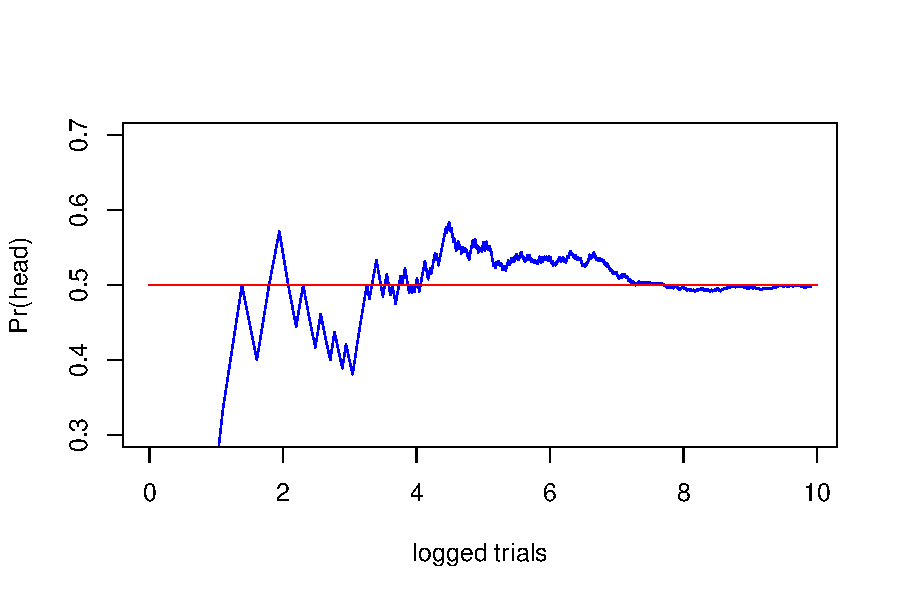
\includegraphics{C:/Users/katoo/Desktop/2020EconometricsTA/II/201009/handout_files/figure-latex/WLLN-1.pdf}
\caption{Simulation Result of WLLN}
\end{figure}

\hypertarget{central-limit-theorem}{%
\subsubsection{Central Limit Theorem}\label{central-limit-theorem}}

The second important theorm is the \textbf{central limit theorem}.
Suppose that \(X_i, \ldots, X_n\) are IID sample with mean \(\mu\) and
variance \(\sigma^2\). This theorem says that the sample mean
\(\bar{X}_n\) has a distribution which is approximately normal with mean
\(\mu\) and variance \(\sigma^2/n\). This theorem does not assume the
distribution of \(X_i\), except the existence of the mean and variance.
Formally,

\begin{quote}
Let \(X_1, \ldots, X_n\) be IID with mean \(\mu\) and variance
\(\sigma^2\). Let \(\bar{X}_n = n^{-1} \sum_{i=1}^n X_i\). Then,
\begin{align*}
Z_n \equiv \frac{\bar{X}_n - \mu}{\sqrt{V(\bar{X}_n)}} = \sqrt{n}\frac{\bar{X}_n - \mu}{\sigma} \stackrel{d}{\to} Z,
\end{align*} where \(Z \sim N(0, 1)\). In other words,
\(\bar{X}_n \stackrel{d}{\to} N(\mu, \sigma^2/n)\).
\end{quote}

As an illustlation, consider a fair coin toss. The random variable is
the number of heads. This random variable has the Bernoulli distribution
with mean \(\mu = 0.5\) and variance \(\sigma^2 = 0.5(1 - 0.5) = 0.25\).
Since we know \(\mu\) and \(\sigma^2\), we can calculate \(Z_n\), using
the sample mean \(\bar{X}_n\). We work this and plot its distribution,
using R programming. We generate 10,000 sample means \(\bar{X}_n\) for
\(n = 3, 5, 100, 1000\), and transform sample means to \(Z_n\). To
calculate \(Z_n\), we use command \texttt{sqrt()}, which returns the
saquare root value. Sometimes, this procedure is called Monte-Carlo
simulation.

\begin{Shaded}
\begin{Highlighting}[]
\KeywordTok{set.seed}\NormalTok{(}\DecValTok{120504}\NormalTok{)}
\NormalTok{m \textless{}{-}}\StringTok{ }\DecValTok{10000}\NormalTok{; n \textless{}{-}}\StringTok{ }\KeywordTok{c}\NormalTok{(}\DecValTok{3}\NormalTok{, }\DecValTok{100}\NormalTok{, }\DecValTok{1000}\NormalTok{); p \textless{}{-}}\StringTok{ }\FloatTok{0.5}
\NormalTok{a \textless{}{-}}\StringTok{ }\KeywordTok{seq}\NormalTok{(}\OperatorTok{{-}}\DecValTok{4}\NormalTok{, }\DecValTok{4}\NormalTok{, }\FloatTok{.01}\NormalTok{); b \textless{}{-}}\StringTok{ }\KeywordTok{dnorm}\NormalTok{(a)}

\NormalTok{dt \textless{}{-}}\StringTok{ }\KeywordTok{list}\NormalTok{(}\StringTok{"n = 3"}\NormalTok{=}\KeywordTok{numeric}\NormalTok{(m), }\StringTok{"n = 100"}\NormalTok{=}\KeywordTok{numeric}\NormalTok{(m), }\StringTok{"n = 1000"}\NormalTok{=}\KeywordTok{numeric}\NormalTok{(m))}
\ControlFlowTok{for}\NormalTok{ (i }\ControlFlowTok{in} \DecValTok{1}\OperatorTok{:}\DecValTok{3}\NormalTok{) \{}
\NormalTok{  dt[[i]] \textless{}{-}}\StringTok{ }\KeywordTok{rbinom}\NormalTok{(}\DataTypeTok{n =}\NormalTok{ m, }\DataTypeTok{size =}\NormalTok{ n[i], }\DataTypeTok{prob =}\NormalTok{ p)}
\NormalTok{  dt[[i]] \textless{}{-}}\StringTok{ }\KeywordTok{sqrt}\NormalTok{(n[i])}\OperatorTok{*}\NormalTok{(dt[[i]]}\OperatorTok{/}\NormalTok{n[i] }\OperatorTok{{-}}\StringTok{ }\NormalTok{p)}\OperatorTok{/}\KeywordTok{sqrt}\NormalTok{(p}\OperatorTok{*}\NormalTok{(}\DecValTok{1}\OperatorTok{{-}}\NormalTok{p))}
\NormalTok{\}}

\KeywordTok{par}\NormalTok{(}\DataTypeTok{mfrow=}\KeywordTok{c}\NormalTok{(}\DecValTok{2}\NormalTok{,}\DecValTok{2}\NormalTok{), }\DataTypeTok{mai =} \KeywordTok{c}\NormalTok{(}\FloatTok{0.5}\NormalTok{, }\FloatTok{0.5}\NormalTok{, }\FloatTok{0.35}\NormalTok{, }\FloatTok{0.35}\NormalTok{)) }
\ControlFlowTok{for}\NormalTok{ (i }\ControlFlowTok{in} \DecValTok{1}\OperatorTok{:}\DecValTok{3}\NormalTok{) \{}
  \KeywordTok{hist}\NormalTok{(dt[[i]], }\DataTypeTok{col =} \StringTok{"grey"}\NormalTok{, }\DataTypeTok{freq =} \OtherTok{FALSE}\NormalTok{, }
    \DataTypeTok{xlab =} \StringTok{""}\NormalTok{, }\DataTypeTok{main =} \KeywordTok{names}\NormalTok{(dt)[i], }\DataTypeTok{xlim =} \KeywordTok{c}\NormalTok{(}\OperatorTok{{-}}\DecValTok{4}\NormalTok{, }\DecValTok{4}\NormalTok{))}
  \KeywordTok{par}\NormalTok{(}\DataTypeTok{new =} \OtherTok{TRUE}\NormalTok{)}
  \KeywordTok{plot}\NormalTok{(a, b, }\DataTypeTok{type =} \StringTok{"l"}\NormalTok{, }\DataTypeTok{col =} \StringTok{"red"}\NormalTok{, }\DataTypeTok{axes =} \OtherTok{FALSE}\NormalTok{, }
    \DataTypeTok{xlab =} \StringTok{""}\NormalTok{, }\DataTypeTok{ylab =} \StringTok{""}\NormalTok{, }\DataTypeTok{main =} \StringTok{""}\NormalTok{)}
\NormalTok{\}}
\end{Highlighting}
\end{Shaded}

\begin{figure}
\centering
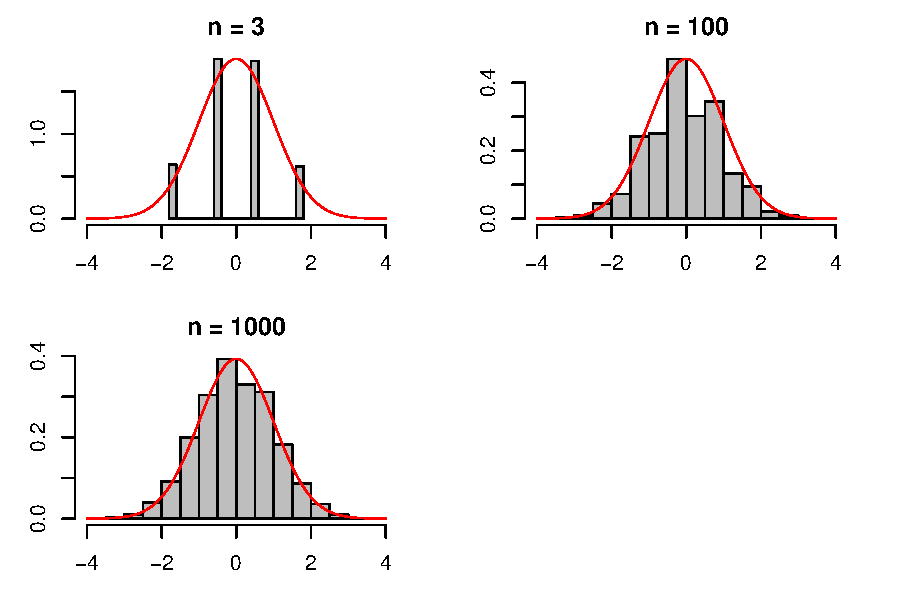
\includegraphics{C:/Users/katoo/Desktop/2020EconometricsTA/II/201009/handout_files/figure-latex/CLT-1.pdf}
\caption{Simulation Result of CLT}
\end{figure}

\hypertarget{review-linear-regression}{%
\section{Review: Linear Regression}\label{review-linear-regression}}

This section refers to Johnston (1984) and Angrist and Pischke (2008).
Consider the \(k\)-variables lienar regression model: \begin{align*}
  y_i = x_i \beta + u_i,
\end{align*} where \(\beta = (\beta_0, \beta_1, \ldots, \beta_k)'\) is a
\(k \times 1\) vector of regression coefficients,
\(x_i = (1, x_{i1}, \ldots, x_{ik})\) is a \(1 \times k\) vector of
stochastic covariates, and \(u_i\) is the error term which is idependent
and identically distributed (i.i.d.). Our parameter of interest is
\(\beta\).

\hypertarget{ordinary-least-squares-estimator-olse}{%
\subsection{Ordinary Least Squares Estimator
(OLSE)}\label{ordinary-least-squares-estimator-olse}}

The \textbf{OLS estimators} are the value \(\beta\) such that minimizing
the residual sums of squares, that is,

\begin{quote}
The \textbf{OLS estimators} \(\hat{\beta}\) is defined by \begin{align*}
\hat{\beta} \in \mathop{\rm arg~min}\limits_{\beta} \sum_{i = 1}^n (y_i - x_i \beta)^2,
\end{align*} or, \begin{align*}
\hat{\beta} \in \mathop{\rm arg~min}\limits_{\beta} (Y - X \beta)'(Y - X \beta),
\end{align*} where \(Y = (y_1, \ldots, y_n)'\) is a \(n \times 1\)
vector, and \(X = (x_1, \ldots, x_n)'\) is a \(n \times k\).
\end{quote}

Following this definition, the OLSE is given by \begin{align*}
  \hat{\beta} = (X'X)^{-1}(X'Y).
\end{align*} To exist the inverse matrix, we assume that the matrix
\((X'X)\) is the regular matrix (i.e., there is no perfect correlation
between any two covariates).

\hypertarget{best-linear-unbiased-estimator-blue}{%
\subsubsection{Best Linear Unbiased Estimator
(BLUE)}\label{best-linear-unbiased-estimator-blue}}

We impose assumptions about the disturbance vector \(u\): (i)
\(E(u|X) = 0\) (exogenity assumption or mean-idependence), and (ii)
\(V(u|X) = \sigma^2 I\) (homoscedasticity and pairwise uncorrelation).
Under this condition, the OLS estimator is a linear unbiased estimator,
that is, \(E(\hat{\beta}) = \beta\) since \begin{align*}
  E(\hat{\beta}|X) = E[\beta + (X'X)^{-1}(X'u)|X] = \beta + (X'X)^{-1}X'E(u|X) = \beta.
\end{align*} Furthermore, the variance-covariance matrix of OLSE is
\begin{align*}
  V(\hat{\beta}|X) 
  &= E[(X'X)^{-1}X' uu' X (X'X)^{-1} | X] \\
  &= (X'X)^{-1}X' \sigma^2 I X (X'X)^{-1} \\
  &= \sigma^2 (X'X)^{-1}.
\end{align*} Note that \(V(\hat{\beta}) = \sigma^2 E[ (X'X)^{-1} ]\).
The most important result is that no other linear unbiased estimator can
have smaller variances than those of OLSE. In other words, the OLSE has
minimum variance within the class of linear unbiased estimators. Thus,
the OLSE is a best linear unbiased estimator (\textbf{BLUE}). This
result is known as the \emph{Gauss-Markov theorem} (We omit proof).

\hypertarget{asymptotic-properties}{%
\subsubsection{Asymptotic Properties}\label{asymptotic-properties}}

First, the OLSE is a consistent estimator, that is, \begin{align*}
  \mathop{\mathrm{plim}}\hat{\beta} = \beta + \mathop{\mathrm{plim}}\left( \frac{1}{n} (X'X) \right)^{-1} \mathop{\mathrm{plim}}\left( \frac{1}{n} X'u \right) = \beta.
\end{align*} This is bacause
\(\mathop{\mathrm{plim}}n^{-1} (X'X) = \mathop{\mathrm{plim}}n^{-1} \sum_i x'_i x_i = E[x'_i x_i] = \Sigma\)
and
\(\mathop{\mathrm{plim}}n^{-1} (X'u) = \mathop{\mathrm{plim}}n^{-1} \sum_i x'_i u_i = E[x'_i u_i] = 0\)
by mean-independence assumption.

Second, the OLSE is asymptotically normally distributed. To show it, we
derive the asymptotic distribution of \(\sqrt{n}(\hat{\beta} - \beta)\)
where \begin{align*}
  \sqrt{n}(\hat{\beta} - \beta) = \left( \frac{1}{n} \sum_i x'_i x_i \right)^{-1} \sqrt{n} \left( \frac{1}{n} \sum_i x'_i u_i \right).
\end{align*} By the central theorem, we have \begin{align*}
  \sqrt{n} \left( \frac{1}{n} \sum_i x'_i u_i \right) \overset{d}{\to} N(0, \sigma^2 \Sigma).
\end{align*} Recall that
\(n^{-1} \sum_i x'_i x_i \overset{p}{\to} \Sigma\). By the Slutsky
theorem (the 6th property of convergence), we get \begin{align*}
  \sqrt{n}(\hat{\beta} - \beta) \overset{d}{\to} N(0, \sigma^2 \Sigma^{-1}),
\end{align*} or, \begin{align*}
  \hat{\beta} \overset{d}{\to} N \left(\beta, \frac{1}{n} \sigma^2 \Sigma^{-1} \right).
\end{align*}

In a practical application, the unknown \(\Sigma\) is replaced by the
sample estimate \(n^{-1} X'X\), and the unknown \(\sigma^2\) is
estimated by \(\hat{\sigma}^2 = \hat{u}'\hat{u}/(n-k)\) where
\(\hat{u} = Y - X \hat{\beta} = (I_n - X(X'X)^{-1}X')u = M_X u\) and
\(M_X\) is a symmetric and idempotent matrix. Note that
\(\hat{\sigma}^2\) is an unbiased estimator of \(\sigma^2\) since
\begin{align*}
  E[ \hat{\sigma}^2 ] = \frac{1}{n-k} E[tr(M_X uu')] = \frac{\sigma^2}{n-k} tr(M_X I_n) = \sigma^2. 
\end{align*}

\hypertarget{finite-sample-distribution-and-inference}{%
\subsubsection{Finite-sample Distribution and
Inference}\label{finite-sample-distribution-and-inference}}

Now, we add the assumption with respect to the error term,
\(\epsilon_i |x_i \overset{iid}{\sim} N(0, \sigma^2)\). Then, we
immediately obtain \begin{align*}
  \hat{\beta}|X \sim N(\beta, \sigma^2(X'X)^{-1}).
\end{align*}

Consider the set of linear null hypothesis embodied in \(R \beta = r\)
where \(R\) is a arbitrary \(q \times k\) matrix and \(r\) is a known
\(q\)-element vector. To develop a test procedure, we derive the exact
distribution of \(R\hat{\beta}\). Cleary, we see
\(E(R\hat{\beta}) = R\beta\) and
\(V(R\hat{\beta}) = \sigma^2 R (X'X)^{-1} R'\). This leads to
\begin{align*}
  R(\hat{\beta} - \beta) \sim N(0, \sigma^2 R (X'X)^{-1} R').
\end{align*} If the null hypothesis is true, then \begin{align*}
  R\hat{\beta} - r \sim N(0, \sigma^2 R (X'X)^{-1} R').
\end{align*} Using it and \(\hat{u}'\hat{u} = u' M_X u\), we have
follwing two distributions \begin{align*}
  &(R\hat{\beta} - r)'[\sigma^2 R (X'X)^{-1} R']^{-1}(R\hat{\beta} - r) \sim \chi^2(q),  \\
  &\frac{\hat{u}'\hat{u}}{\sigma^2} \sim \chi^2(n - k)
\end{align*} To derive these distributions, we use the following two
properties about chi-squared distribution:

\begin{itemize}
\tightlist
\item
  If \(x \sim N(0, \Sigma)\), then \(x'\Sigma x \sim \chi^2(n)\) where
  \(x\) is \(n\)-element vector.
\item
  If \(x \sim N(0, \sigma^2 I)\) and \(A\) is idempotent matrix, then
  \((\sigma^2)^{-1} x'Ax \sim \chi^2(tr(A))\).
\end{itemize}

Finally, since \(X_1 \sim \chi^2(d_1)\) and \(X_2 \sim \chi^2(d_2)\)
lead to \(\frac{X_1}{d_1}/\frac{X_2}{d_2} \sim F(d_1, d_2)\), we have
the distribution of test statistic, called the F-distribution,
\begin{align*}
  \frac{(R\hat{\beta} - r)'[R (X'X)^{-1} R']^{-1}(R\hat{\beta} - r)/q}{\hat{u}'\hat{u}/(n - k)} \sim F(q, n-k).
\end{align*} The test procedure is to reject the null hypothesis
\(R\beta = r\) if the computed F-value exceeds a preselected cricial
value.

Especially, when we test a single coefficient, we can use the t-value as
an alternative test statistic. Suppose that \(R = (0, 1, 0, \ldots, 0)\)
and \(r = 0\). The null hypothesis is \(\hat{\beta}_2 = 0\). The matrix
\(R (X'X)^{-1} R'\) picks up the second diagonal element of
\((X'X)^{-1}\) denoted by \((X'X)^{-1}_{22}\). Then, we have
\begin{align*}
  \frac{\hat{\beta}_2^2}{\hat{\sigma}^2 (X'X)^{-1}_{22}} \sim F(1, n-k).
\end{align*} Since \(t \sim t(n)\) is equivalent to \(t^2 \sim F(1, n)\)
for any \(n\), we finally obtain the test statistic following the
Student's t-distribution \begin{align*}
  \frac{\hat{\beta}_2}{\hat{\sigma} \sqrt{(X'X)^{-1}_{22}}} \sim t(n - k).
\end{align*} When you use t-test of a single coefficient, you should
\emph{two-sided} t-test. If the computed t-statistic \(\hat{t}\) holds
\(|\hat{t}| > t_{1-\alpha/2}(n-k)\) where \(t_{q}(n-k)\) is the
\(q\)-percentile t-value, then we can reject the null hyporhesis
\(\hat{\beta}_2 = 0\)

\hypertarget{maximum-likelihood-estimator-mle}{%
\subsection{Maximum Likelihood Estimator
(MLE)}\label{maximum-likelihood-estimator-mle}}

When we assume that the error term is normally distributed, we have
\(y_i | x_i \overset{iid}{\sim} N(x_i \beta, \sigma^2)\). Under this
assumption, the estimator \(\tilde{\beta}\) maximizing the
log-likelihood function, called \textbf{maximum likelihood estimator},
is equivalent to the OLSE. The likelihood function is \begin{align*}
  \prod_{i=1}^n f(y_i, x_i)
  = \prod_{i=1}^n f_{Y|X}(y_i | x_i) \prod_{i=1}^n f_X(x_i)
  = \sum_{i=1}^n \log f_{Y|X}(y_i | x_i) + \sum_{i=1}^n \log f_X(x_i).
\end{align*} Since \(f_X(x_i)\) does not involve the parameter vector
\(\beta\), the \emph{conditional} MLE \(\tilde{\beta}\) maximizes the
conditional log-likelihood function
\(\sum_{i=1}^n \log f_i(y_i | x_i)\), that is, \begin{align*}
  \log L(\theta) 
  &= \sum_{i=1}^n \log f_{Y|X}(y_i | x_i)  \\
  &= \sum_{i=1}^n \log \left( (2\pi\sigma^2)^{-1/2} \exp\left( -\frac{(y_i - x_i \beta)^2}{2\sigma^2} \right) \right)  \\
  &= -\frac{n}{2} \log (2\pi) -\frac{n}{2}\log\sigma^2 -\frac{1}{2\sigma^2} (Y - X \beta)'(Y - X \beta),
\end{align*} where \(\theta = (\beta', \sigma^2)'\) is a
\((k + 1) \times 1\) vector of unknown parameters. The first-order
derivatives of this function, sometimes called \textbf{score}, is given
by \begin{align*}
  \frac{\partial \log L(\theta)}{\partial \theta} =
  \begin{pmatrix}
    -\frac{1}{2\sigma^2} (-2X'Y + 2X'X \beta) \\
    -\frac{1}{2\sigma^2} \left(n - \frac{1}{\sigma^2} (Y - X \beta)'(Y - X \beta) \right)
  \end{pmatrix}.
\end{align*} The necessary condition of MLE is
\(\frac{\partial}{\partial \theta} \log L(\theta) = 0\). This leads to
the following MLE: \begin{align*}
  \tilde{\beta} = (X'X)^{-1}(X'Y),\quad \tilde{\sigma}^2 = \frac{\hat{u}'\hat{u}}{n}.
\end{align*} The sufficient condition of MLE is the following Hessian
matrix is negative definite. \begin{align*}
  H(\theta) =
  \begin{pmatrix}
    -\frac{1}{\sigma^2} X'X  & \frac{1}{2\sigma^4} (-X'Y + X'X \beta) \\
    \frac{1}{2\sigma^4} (-X'Y + X'X \beta) & \frac{n}{2\sigma^4} - \frac{1}{\sigma^6} (Y - X \beta)'(Y - X \beta)
  \end{pmatrix}.
\end{align*}

\hypertarget{properties-of-mle}{%
\subsubsection{Properties of MLE}\label{properties-of-mle}}

First, we provide the \emph{Cramer-Rao theorem} that states that ML
methods gives the lower bound of variance of unbiased estimators (proof
is omitted).

\begin{quote}
Let \(\tilde{\theta}\) denote an unbiased estimator of \(\theta\). Then,
\(V(\tilde{\theta}) - I^{-1}(\theta)\) is a positive definite where
\(I(\theta)\) is a \textbf{Fisher information matrix}, which is defined
by \begin{align*}
I(\theta) 
= - E (H(\theta)) 
= - E 
\begin{pmatrix}
\frac{\partial^2 \log L(\theta) }{\partial \theta_1^2} &
\frac{\partial^2 \log L(\theta) }{\partial \theta_1 \partial \theta_2} &
\cdots &
\frac{\partial^2 \log L(\theta) }{\partial \theta_1 \partial \theta_k} \\
\frac{\partial^2 \log L(\theta) }{\partial \theta_2 \partial \theta_1} &
\frac{\partial^2 \log L(\theta) }{\partial \theta_2^2} &
\cdots &
\frac{\partial^2 \log L(\theta) }{\partial \theta_2 \partial \theta_k} \\
\vdots & \vdots & \vdots & \vdots \\
\frac{\partial^2 \log L(\theta) }{\partial \theta_k \partial \theta_1} &
\frac{\partial^2 \log L(\theta) }{\partial \theta_k \partial \theta_2} &
\cdots &
\frac{\partial^2 \log L(\theta) }{\partial \theta_k^2}
\end{pmatrix}.
\end{align*}
\end{quote}

Note that the Fisher information matrix conditional on some random
variables also provides the Cramer-Rao lower bound. In the case of
linear regression, the Cramer-Rao lower bound condtional on \(X\) gives
\begin{align*}
  I^{-1} \begin{pmatrix} \beta \\ \sigma^2 \end{pmatrix}
  = 
  \begin{pmatrix} \sigma^2 X'X^{-1} & 0 \\ 0 & \frac{2\sigma^4}{n} \end{pmatrix}.
\end{align*} Although the ML estimator of \(\beta\) attains the
Cramer-Rao lower bound, the ML estimator of \(\sigma^2\) deviates.

Second, we summarize asymptotic properties of MLE as follows (proof is
omitted):

\begin{quote}
Under certain regularity conditions, (i) The ML estimator is consistent,
i.e., \(\tilde{\theta} \overset{p}{\to} \theta\), and (ii) The ML
estimator is asymptotically normally distributed, i.e.,
\(\tilde{\theta} \overset{d}{\to} N(\theta, I^{-1}(\theta))\)
\end{quote}

\hypertarget{reference}{%
\section*{Reference}\label{reference}}
\addcontentsline{toc}{section}{Reference}

\hypertarget{refs}{}
\begin{cslreferences}
\leavevmode\hypertarget{ref-angrist2008mostly}{}%
Angrist, Joshua D, and Jörn-Steffen Pischke. 2008. \emph{Mostly Harmless
Econometrics: An Empiricist's Companion}. Princeton university press.

\leavevmode\hypertarget{ref-johnston1984econometric}{}%
Johnston, J. 1984. \emph{Econometric Methods 3rd}. McGraw-Hill book co.

\leavevmode\hypertarget{ref-wasserman2013all}{}%
Wasserman, Larry. 2013. \emph{All of Statistics: A Concise Course in
Statistical Inference}. Springer Science \& Business Media.
\end{cslreferences}

\end{document}
